\section{くりくり$\heartsuit$せんけーだいすーにゅうもん♪}
% この章では線形代数の入門を行う。以下の習得を目的とする
% ベクトルの基本性質(足し算、スカラー、内積)、行列の基本性質(足し算、掛け算、単位行列、転置、ユニタリ行列)、線形写像、逆行列、行列式について学ぶ
%
\subsection{ベクトル}
\subsubsection{平面ベクトルの定義と演算}
\ \\
% 漫画は定義と意味をさらっとおさらいする感じ。後ろの文章のところで詳しく解説する。
\kao{fig/holmy.png}{まずは、機械学習を議論する上で最も重要となるベクトルと行列を学びます}\\
\kao{fig/jacklyn.png}{ベクトル? 『チームのベクトル』みたいに使うし、向きって意味やっけ?}\\
\kaot{fig/holmy.png}{そうですね、{\bf ベクトル}とは向きと大きさを表すもので、例えば二次元平面なら$(x_1, x_2)\ (x_1,x_2 \in \mathbb{R})$という実数の組で記載します。\\
今回は簡単のため実数の集まり(${\mathbb{R}}$)のみを考え、$x_1$が実数である、つまり実数集合の一つという意味で$x_1\in \mathbb{R}$と書きます。}\\
\[
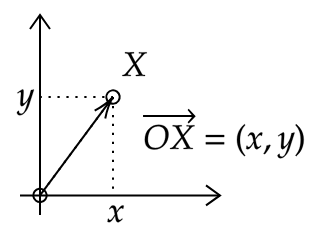
\includegraphics[width=4cm]{fig/1_1_vector.png}
\]
\kaot{fig/holmy.png}{ベクトルは例えば、原点$(0,0)$から$(x_1,x_2)$の点への矢印を表すものです。
今は点とベクトルを区別するため、点は大文字アルファベット$A,B,\cdots$で表し、ベクトルは$\vecbold{a},\vecbold{b},...$と小文字アルファベット太文字で表します。
特に原点は$O$,点$A$から点$B$へのベクトルを$\overrightarrow{AB}$と書きます。
最初はわかりやすく2次元平面で話していきますね。}\\
\kao{fig/rosia.png}{ふーん、矢印ねぇ…でも、矢印って平面上にいっぱいない? 同じものもあると思うんだけど、それって区別できるの??}\\
\kaot{fig/holmy.png}{いいところに気が付きましたね! 違う地点からの{\bf 矢印でも向きと長さ($(x_1, x_2)$の組)が同じものは同じと見なして一つのもの}とします。
% ベクトルの演算と同値なベクトルの関係、ベクトルの演算と=は両立する
さてここで、点$O=(0,0)$から点$A=(1,1)$へのベクトル$\overrightarrow{OA}$と点$B=(1,0)$から点$C=(2,1)$へのベクトル$\overrightarrow{BC}$を考えてみましょう。}\\
\kao{fig/rosia.png}{どっちも$(1,1)$じゃないの?}\\
\kaot{fig/holmy.png}{その通りです。ここで、$\overrightarrow{BC}$を始端の点と終端の点が同じのベクトル同士をつなげることを$+$で表して、考えると
\[
    (1,1)=\overrightarrow{BC}=\overrightarrow{BO}+\overrightarrow{OC}=(-1,0)+(2,1)
\]
となります。($\overrightarrow{BO}$は$\overrightarrow{OB}=(1,0)$の逆向きなので$(-1,0)$)}\\
\[
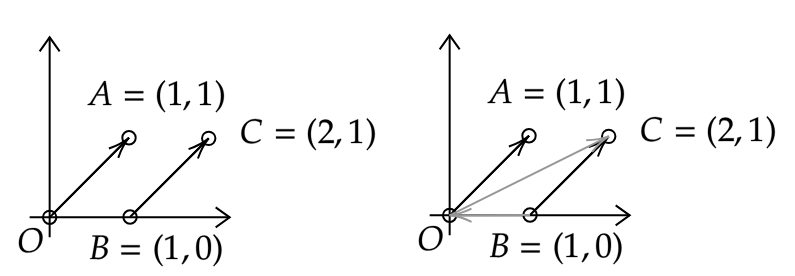
\includegraphics[width=8cm]{fig/1_1_vector_sum_bw.png}
\]
\kao{fig/tsukino.png}{えーっと、これって右の足し算が$(-1,0)+(2,1)$が$(-1+2,0+1)=(1,1)$になってるの…?}\\
\kaot{fig/holmy.png}{はい! このようにベクトル同士の足し算は次のように定義します
\[
    (x_1,x_2)+(y_1,y_2) := (x_1+y_1,x_2+y_2).
\]
また、ベクトルは同じ矢印の向きと長さが同じものを一つに見なしてたので、$(y_1,y_2)$の矢印を始端を$(x_1,x_2)$の終端に合わせることができ、すべてのベクトルに対して足し算を考えることができます。}\\
% TODO: ベクトルの和の例を図示
\kao{fig/tsukino.png}{ええっと、つまり、前の矢印に後ろの矢印を持ってきてあげるの…あれ、どっちも同じになるの}\\
\kao{fig/holmy.png}{ツキノの言う通り、ベクトルの足し算には以下の性質が成り立ちます。}
\begin{breakbox}
    \begin{Prop}
        \label{Prop1_1_1}
        $\vecbold{o}=(0,0)$として、任意のベクトル$\vecbold{a},\vecbold{b},\vecbold{c}$について
        \begin{enumerate}[$(1)$]
            \item $\vecbold{a}+\vecbold{b}=\vecbold{b}+\vecbold{a}$ (交換律)
            \item $(\vecbold{a}+\vecbold{b})+\vecbold{c}=\vecbold{a}+(\vecbold{b}+\vecbold{c})$ (交換律)
            \item $\vecbold{a}+\vecbold{o}=\vecbold{a}$
        \end{enumerate}
    \end{Prop}
\end{breakbox}
\[
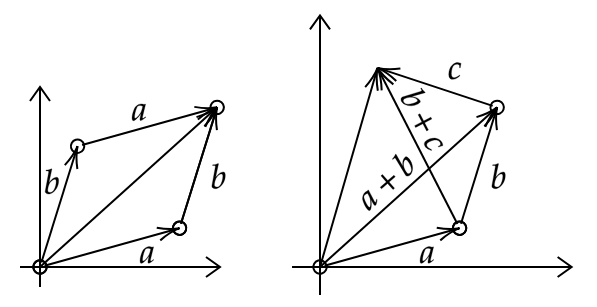
\includegraphics[width=8cm]{fig/1_1_vector_sum2.png}
\]
\ \\
\kaot{fig/holmy.png}{さて、次にベクトルの引き算を考えてみます。$\overrightarrow{OA}=(x_1,x_2)$に対して、
\[
    \overrightarrow{AO}+(-\overrightarrow{AO})=(0,0) \Rightarrow -\overrightarrow{AO}=(-x_1,-x_2)
\]
また、$\overrightarrow{AO}+\overrightarrow{OA}=(0,0)$なので、$-\overrightarrow{AO}=\overrightarrow{OA}$となります。
このマイナスの定義をよく見ると、元のベクトルの中身に$-1$をかけてます。}\\
\kao{fig/rosia.png}{いわれてみればそうね}\\
\kaot{fig/holmy.png}{これはベクトルの長さ$-1$倍していると考えることができます。これを一般化して実数$c$についてベクトルを$c$倍することを考えます。ベクトル$(x_1,x_2)$の$c$倍は
\[
    c(x_1,x_2) := (cx_1,cx_2)
\]
となり、これを{\bf スカラー倍}といいます。スカラー倍には次の性質が成立します。}
\begin{breakbox}
    \begin{Prop}
        \label{Prop1_1_2}
        任意のベクトル$\vecbold{a},\vecbold{b}$,実数$c,d$について、
        \begin{enumerate}[$(1)$]
            \item $c(\vecbold{a}+\vecbold{b})=c\vecbold{a}+c\vecbold{b}$
            \item $(c+d)\vecbold{a}=c\vecbold{a}+d\vecbold{a}$
            \item $(cd)\vecbold{a}=c(d\vecbold{a})$
            \item $1\vecbold{a} = \vecbold{a}$
        \end{enumerate}
    \end{Prop}
\end{breakbox}
\ \\
\kao{fig/holmy.png}{さて、続いて、次にベクトルの長さを定義します。ベクトル$\vecbold{x}=(x_1,x_2)$の長さ、つまり、$(0,0)$から$(x_1,x_2)$の距離になります。}\\
\kaot{fig/rosia.png}{あっ、これどこかで聞いたことある。\footnotemark[1]たしか三平方の定理から
\[
    \sqrt{(0-x_1)^2+(0-x_2)^2}=\sqrt{x_1^2+x_2^2}
\]
じゃない?}
\footnotetext[1]{ろーほるすーがくれっすん \S 3
\\ \url{https://irisu-in-wonderland.tumblr.com/post/156533872627}}\\
\kaot{fig/holmy.png}{その通りです! ベクトルの$\vecbold{x}=(x_1,x_2)$の長さをベクトルのノルムと言い、$\|\vecbold{x}\|$と表し
\[
    \|\vecbold{x}\| = \sqrt{x_1^2+x_2^2}
\]
となります。もちろんベクトルの引き算の定義から
\[
    \|\vecbold{x}-\vecbold{y}\| = \|(x_1-y_1,x_2-y_2)\| = \sqrt{(x_1-y_1)^2+(x_2-y_2)^2}
\]
となり、$\|\vecbold{x}-\vecbold{y}\|$は$(x_1,x_2)$と$(y_1,y_2)$の距離となります。}\\
\kao{fig/rosia.png}{まあ、確かにベクトルの引き算から距離っぽくなるよね。}\\
\kaot{fig/holmy.png}{続いて、ベクトル同士の角度を表すことができる{\bf 内積}を定義します。ベクトル$\vecbold{x},\vecbold{y}$の内積を$\vecbold{x}\cdot\vecbold{y}$と表し、
\[
    \vecbold{x}\cdot\vecbold{y} := x_1 \times y_1 + x_2 \times y_2
\]
もちろん、定義から$\vecbold{x}$のノルムは内積を使って
\[
    \|\vecbold{x}\| = \sqrt{\vecbold{x}\cdot\vecbold{x}}
\]
となります。}\\
\kao{fig/rosia.png}{うーん…これのどこが角度と関係するの?}\\
\kaot{fig/holmy.png}{簡単な例で考えてみましょう。\\
長さが1のベクトル$\vecbold{x},\vecbold{y}$を考えます。$\vecbold{x},\vecbold{y}$は長さが1なので原点を中心とした半径1の円のどこかに位置します。\\
ここで、$\vecbold{x}=(1,0)$として、円上のベクトル$\vecbold{y}$を考えてると、$\vecbold{x}$と$\vecbold{y}$の角度$\theta$として、$\vecbold{y}=(\cos \theta,\sin \theta)$と書けます。}\\
\[
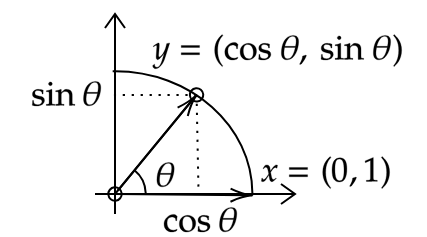
\includegraphics[width=6cm]{fig/1_1_sincos.png}
\]
\kaot{fig/holmy.png}{このとき
\[
    \vecbold{x}\cdot\vecbold{y} = \cos \theta
\]
となります。このように内積は角度$\theta$についての関数$\cos$と関係してます。\\
ただし、この$\theta$は角度ですが、1回転が$360^\circ$で表記せず、1回転が$2\pi$,$180^\circ$が$\pi$と半径1の円の弧に対応する{\bf 弧度法}を使用します。}\\
\kao{fig/jacklyn.png}{こどほう…? 波動砲みたいやな??}\\
\kao{fig/rosia.png}{ふーん、円の長さを角度とみるんだ、なんだか馴染みないわね。}\\
\kaot{fig/holmy.png}{実は、こうした方が都合が良いことがわかります\footnotemark[1]。以下に度数法と弧度法の対応する表を載せておきます。
\[
    \begin{tabular}{|l|l|l|l|} \hline
        度数法 & $360^\circ$ & $180^\circ$ & $90^\circ$ \\ 
        弧度法 & $2\pi$ & $\pi$ & $\frac{\pi}{2}$ \\ \hline
    \end{tabular}
\]
さて、一般的なベクトルに対して
\[
    \cos \theta = \frac{\vecbold{x}\cdot\vecbold{y}}{\|x\|\|y\|}
\]
が成立します。}
\footnotetext[1]{微分を用いると$(\cos \theta)^\prime = \sin\theta$となるが、今度数法で三角関数を定めると$\cos _{a}\theta = \cos \frac{\pi}{180}\theta$とすると\S 2.2で示す合成関数の微分より
$(\cos _{a}\theta)^\prime = \frac{\pi}{180}\sin \frac{\pi}{180}\theta$となり、微分する度余計な定数が出てきて都合が悪い。}\\
% TODO: 図
\kao{fig/jacklyn.png}{そう言われてみれば角度っぽいなぁ…}\\
\kaot{fig/holmy.png}{ただこの説明で、何でもいいから円上の点へのベクトル$\vecbold{x},\vecbold{y}$を$\vecbold{x}=(1,0)$として、
円上のベクトル$\vecbold{y}$で考えた部分は、内積がベクトルを$t$回転させる関数$f_t$について変わらないことを言わないといけないです。つまり、
\[
\vecbold{x}\cdot\vecbold{y}=f_t(\vecbold{x})\cdot f_t(\vecbold{y})    
\]
が成立します。\\
次にどんなベクトル$\vecbold{x}=(x_1,x_2)$もベクトル$\vecbold{e_1}=(1,0),\vecbold{e_2}=(0,1)$として
\[
    \vecbold{x}=x_1\vecbold{e_1}+x_2\vecbold{e_2}
\]
となります。では、$\vecbold{e_1},\vecbold{e_2}$だけでなく他の2つのベクトルで平面すべてを表すことを考えます。}\\
\kao{fig/rosia.png}{他のベクトルで平面を表すってそんな簡単にできるの?}\\
\kaot{fig/holmy.png}{実は意外に簡単で、2つのベクトル$\vecbold{a},\vecbold{b}$が平行でなければ良いです。すると、$\vecbold{a},\vecbold{b}$のベクトルで平行四辺形を作ることが出来、
その平行四辺形を左右上下に張り付けていけば、全ての平面を覆うことが出来ると考えられます。
ここで$\vecbold{a},\vecbold{b}$が平行でないを式で表すと$\vecbold{a}=k\vecbold{b}$となる実数$k$が存在しないことであり、これは方程式
\[
    c_1\vecbold{a}+c_2\vecbold{b}=0
\]
の解$(c_1,c_2)$が$(0,0)$のみであることが言えます。このような平行でないという性質を{\bf 線形独立}といいます。}\\
\kao{fig/jacklyn.png}{平行じゃないだけでそんな性質あるんやなぁ…}
\subsubsection{$n$次元ベクトル}
\ \\
\kao{fig/holmy.png}{さて、これまで2次元のベクトルについて学んできましたが、これを$n$次元に拡張してみます。機械学習に使う数学では$n$次元を扱うので、$n$次元ベクトルを定義します。}\\
\kao{fig/tsukino.png}{$n$次元…全然想像できないの…}\\
\kao{fig/holmy.png}{まあ、私たちは3次元しか見えてないのでイメージしにくいと思います…しかし、定義は非常に明快です。}\\
\kao{fig/jacklyn.png}{もしかして、2次元のときは2つの数の組だったんやから、$n$次元の場合は$n$個の数があればええんとちゃう?}\\
\kaot{fig/holmy.png}{ジャクリン、正解です! $n$次元のベクトル$\vecbold{x}$は以下のように定義します。
\[
    \vecbold{x}=(x_1,x_2,\cdots,x_n)\ \ (x_1,x_2,\cdots,x_n \in \mathbb{R})
\]
そして、$n$次元ベクトル$\vecbold{x}=(x_1,x_2,\cdots,x_n),\vecbold{y}=(y_1,y_2,\cdots,y_n)$,$c\in \mathbb{R}$について、足し算とスカラー倍を
\begin{align*}
    &\vecbold{x}+\vecbold{y} = (x_1+y_1,x_2+y_2,\cdots,x_n+y_n)\\
    &c\vecbold{x}=(cx_1,cx_2,\cdots,cx_n)
\end{align*}
と定めます。$\mathbb{R}$の$n$次元ベクトルの集合を$\mathbb{R}^n$と書きます。\\
$n$次元の場合についても2次元の場合と同じように次の命題が成立します。}
\begin{breakbox}
    \begin{Prop}
        \label{Prop1_1_3}
        $\vecbold{o}=(0,0)$として、任意のベクトル$\vecbold{a},\vecbold{b},\vecbold{c}\in \mathbb{R}^n$について
        \begin{enumerate}[$(1)$]
            \item $\vecbold{a}+\vecbold{b}=\vecbold{b}+\vecbold{a}$ (交換律)
            \item $(\vecbold{a}+\vecbold{b})+\vecbold{c}=\vecbold{a}+(\vecbold{b}+\vecbold{c})$ (結合律)
            \item $\vecbold{a}+\vecbold{o}=\vecbold{a}$ 
        \end{enumerate}
    \end{Prop}
\end{breakbox}
\begin{proof}
    $\vecbold{a}=(\cdots,a_i,\cdots),\vecbold{b}=(\cdots,b_i,\cdots),\vecbold{c}=(\cdots,c_i,\cdots)$とかく。すると\\
    交換律:
    \[
        \vecbold{a}+\vecbold{b}=(\cdots,a_i+b_i,\cdots)=(\cdots,b_i+a_i,\cdots)=\vecbold{b}+\vecbold{a},
    \]
    結合率:
    \[
        (\vecbold{a}+\vecbold{b})+\vecbold{c}=(\cdots,a_i+b_i,\cdots)+\vecbold{c}=(\cdots,(a_i+b_i)+c_i,\cdots)=(\cdots,a_i+(b_i+c_i),\cdots)=\vecbold{a}+(\vecbold{b}+\vecbold{c})
    \]
    最後は明らか。
\end{proof}
\ \\
\kaot{fig/holmy.png}{また、$n$次元ベクトルのノルムと内積を次のように定めます。}
\begin{align*}
    \| \vecbold{x} \| &= \sqrt{x_1^2+x_2^2+\cdots+x_n^2}=\sqrt{\sum_{i=1}^n x_i^2} \\
    \vecbold{x}\cdot\vecbold{y} &= x_1y_1+x_2y_2+\cdots+x_ny_n = \sum_{i=1}^n x_i y_i
\end{align*}
\ \\
\kao{fig/tsukino.png}{変なギザギザが出てきたの…}\\
\kao{fig/jacklyn.png}{これはシグマやな~$x_1$から$x_n$を足すときにこう書くんやで~}\\
\kao{fig/tsukino.png}{『シ熊』…ツキノのお仲間さんなの? なんだか仲良くなれそうなの~!}\\
\kao{fig/holmy.png}{違うと思いますが…}\\
\kao{fig/rosia.png}{なんだか、$n$次元ベクトルってどこかで見たことあるのよね~}\\
\kao{fig/holmy.png}{この前、$\sqrt{2}$について教えたときに$n$次元座標は教えたじゃないですか…}\\
\kao{fig/rosia.png}{この前って言ってもずいぶん前のように思えるのは気のせいかしら?}\\
\kaot{fig/holmy.png}{それは言わないお約束です…\\
さて、2次元の時と同様に線形独立が定義されます。ただし、$n$次元の場合は$2\leq k\leq n$の$k$個のベクトル$\vecbold{x}_1,\cdots,\vecbold{x}_k$について
\[
    \sum_{i=1}^k c_i\vecbold{x}_i = 0
\]
となる$(c_1,\cdots,c_k)$が0のみであることを線形独立と言います。}\\
% 点とベクトルは何が違うかを説明する
\kao{fig/rosia.png}{ところでさ、ベクトルと点って何が違うの? 平面だと$(x,y)$という2組の座標で表して、立体だと$(x,y,z)$って3組の座標で表すけど、これってベクトルも同じじゃない?}\\
\kaot{fig/holmy.png}{鋭いところに気が付きましたね! 点とベクトルの違いは、ベクトルには足し算とスカラー倍といった演算があり、
点については演算を言及してないところが大きな違いだと思います。\footnotemark[2]
ベクトルで$n$次元の点を表すことが出来るので、今後は点という言葉を使わずにベクトルのみで考えていきます。}
\footnotetext[2]{点はなんらかの幾何構造を有した空間での要素とベクトルはベクトル空間の要素なので、この説明は語弊があるかもだけど見逃してください…\\
また、点がベクトル表示可能という主張はユークリッドやヒルベルトの公理的幾何学がデカルト座標で表示されることを示さないといけないが、これは『R.ハーツホーン 幾何学 I(丸善出版)』を参照(代数幾何学じゃないよ!)}\\
\kao{fig/rosia.png}{ふーん、まあどっちでもいいってことよね。}\\
\Subsection{ティータイム:一般線形空間}
\begin{minipage}{1.\textwidth}
\font\border=umrandb
\generalframe{\border\char'165}{\border\char'151}{\border\char'164}%
{\border\char'150}{\border\char'150}%
{\border\char'166}{\border\char'151}{\border\char'167}
{
    \centering\bf
ティータイム:一般線形空間
}
\end{minipage}
\ \\
\kao{fig/rosia.png}{ふぅー疲れた。お茶にしようよ。}\\
\kao{fig/holmy.png}{良いですね、お茶のついでに数学の話でも…}\\
\kao{fig/jacklyn.png}{えっ…お茶の時間って休むものなんやないの…?}\\
\kao{fig/rosia.png}{ま、お茶のついでに数学の話をする、そういうものよ。}\\
\kao{fig/holmy.png}{実は、実数の組で表した矢印でなく、曲線や関数などの一般的な対象にも、
足し算とスカラー倍が定められ命題\ref{Prop1_1_1},\ref{Prop1_1_2}と逆ベクトルが唯一つ存在することが言えればベクトルとみなすことができます。}\\
\kao{fig/rosia.png}{んんん??? どういうこと?}\\
\kaot{fig/holmy.png}{ええっと、ベクトルが矢印だけだと似たような性質をもったものに応用できません。\\
実数に留まらず、他にも使えるようにベクトルで大事な性質をまとめて、何らかの集まり$V$に足し算$+:V\times V \to V$(これは$V$と$V$の組に対して$V$への関数という意味)とスカラー体$K$とスカラー倍$\cdot: K\times V \to V$があって、
あるルールを満たすものをベクトルとしようとしてます。}\\
\kaot{fig/holmy.png}{ここで、スカラー体$K$(一般に{\bf 体})とは実数のように足し算$+$と掛け算$\times$が定義されていて、
任意の$a\in K$について$a+o=o$となる0に値するゼロ元、$a\times e=a$となる1に値する単位元などが存在し、$a+(-a)=0$となる$(-a)$がたった一つ存在したり、
$a\neq o$のときに$a\times a^{-1}=e$となる逆数にあたる$a^{-1}$が存在するといった実数の足し算掛け算の性質をもったものです。\\
現代の数学では、ベクトルの集まりはなんでも良く(それこそ猫や椅子でもOK)演算とルールが合えばベクトルで良いとしております。
このような集まり$(V,K,+,\cdot)$を{\bf ベクトル空間(線形空間)}といいます。}\\
\kao{fig/jacklyn.png}{そういうものなんやねぇ~ということはロージアも足し算とスカラー倍が命題\ref{Prop1_1_1},\ref{Prop1_1_2}を満たせばベクトル空間になるってことなん?}\\
\kao{fig/holmy.png}{??? ま、まあそういうことですね…}\\
\begin{breakbox}
    \begin{Def}
        \label{Def1_1_1}
        集合$V$が$K$上のベクトル空間(または線形空間)であるとは、ゼロベクトル$o$、任意のベクトル$x,y,z\in V$、任意のスカラー$a,b\in K$について足し算とスカラー倍が定義されていて、以下が成立することを言う。
        \begin{enumerate}[$(1)$]
            \item $x+y=y+x$ (交換律)
            \item $(x+y)+z=x+(y+z)$ (結合律)
            \item $x+o=x$ 
            \item $x+(-x)=o$となる$-x$が唯一つ存在する
            \item $a\cdot(x+y)=a\cdot x+a\cdot y$ (分配律)
            \item $(a+b)\cdot x=a\cdot x+b\cdot x$ 
            \item $(ab)\cdot x=a\cdot (b\cdot x)$ 
            \item $1\cdot x=x$
        \end{enumerate}
    \end{Def}
\end{breakbox}
\ \\
\kao{fig/rosia.png}{ちょっと定義に隠れて胡麻化そうとしてるけど、私、ベクトルじゃないんだけど}\\
\kao{fig/tsukino.png}{ロージアはベクトルになってもかわいいよ?}\\
\kaot{fig/holmy.png}{そういう問題じゃないと思いますが…\\
えーっと…話を戻しますね…
それまで私たちは$n$次元と言ってましたが、$n$次元はどのように定められるかを考えます。実は線形独立が重要なカギとなっていて、線形独立なベクトルの集まり$A=\{x_1,x_2,\cdots\}\subset V$\footnotemark[1]について
\[
    \{\sum c_ix_i;c_i\in K\} = V
\]
となっているとき$A$を{\bf 基底}といいます。}
\footnotetext[1]{$A \subset B$は集合$A$が$B$に含まれるという意味で、任意の$x\in A$に対して$x\in B$が成立することを言う。}\\
\kao{fig/rosia.png}{つまり、今まで考えてた$\mathbb{R}^n$での$(1,0,\cdots,0)$,$(0,1,\cdots,0)$,$\cdots,(0,0,\cdots,1)$は基底ってことよね。}\\
\kaot{fig/holmy.png}{その通り! これは特に{\bf 標準基底}といい$\vecbold{e_1},\cdots,\vecbold{e_n}$と書きます。\\
そして、一般の線形空間において基底$A$の要素の個数を{\bf 次元}といいます。基底の取り方は色々ありますが、実はその個数は唯一つであることが分かります\footnotemark[2]。\\
とくに$V$の中に線形独立のベクトルが無限に存在する場合、次元は無限になります。}
\footnotetext[2]{斉藤毅 線形代数の世界 定理1.5.4、現代数学概説Iの第6章\S 1定理2を参照。}\\
\kao{fig/tsukino.png}{無限次元…想像つかないの…}\\
\kao{fig/holmy.png}{そうですね、一般の線形空間の例を見てみましょう。有理数$\mathbb{Q}$と実数$\mathbb{R}$は実数$\mathbb{R}$に含まれています($\mathbb{Q}\subset \mathbb{R},\mathbb{R} \subset \mathbb{R}$)
ここで$\mathbb{R}$はその足し算$+$掛け算$\cdot$について、$\mathbb{Q}$上の線形空間、$\mathbb{R}$上の線形空間となってます。}\\
\kao{fig/rosia.png}{ん? 実数が有理数上の線形空間ってことは実数が有理数のベクトルとして見ることができるってこと??}\\
\kaot{fig/holmy.png}{はい、そうです。では、実数を線形空間として見たとき、その次元はどうなるでしょうか? 
$\mathbb{R}$上の線形空間としては1を選んでやれば、どんな実数$x$も$x=x\cdot 1$となり、基底となっているので1次元です。
では、有理数上の実数の線形空間の次元はどうでしょうか? 実は無限次元になります。なぜならば、素数の平方根
\[
    \sqrt{2},\sqrt{3},\sqrt{5},\cdots,\sqrt{p_n},\cdots
\]
が有理数上で線形独立になっているからです。まとめると次の事が言えます。}\\
\begin{breakbox}
    \begin{Prop}
        $\mathbb{R}$は$\mathbb{Q}$上線形空間で、無限次元。
    \end{Prop}
\end{breakbox}
\ \\
\kao{fig/rosia.png}{あれ、これどこかで見たことある…\footnotemark[3]}\\
\footnotetext[3]{「ろーほるすーがくれっすん」の\S 3のスタインハウスの問題を$n$次元に拡張したもの
\\ \url{https://irisu-in-wonderland.tumblr.com/post/156533872627}}
\kaot{fig/holmy.png}{以前のスタインハウスの問題$n$次元を解く点ですね。実はこの問題は素数の平方根の集まりが線形独立であることを本質的に使ってます。
また、$\mathbb{Q}$上の線形空間を考えることで5次以上の方程式には解の公式が存在しないことや、定規とコンパスで何が作図できるかを考えられます。\footnotemark[4]}\\
\footnotetext[4]{E.Artin,Galois Theoryに載っているような現代的なガロア理論のこと。
群はこの研究が初出と言われており、$\mathbb{Q}$の方程式が解ける体$K$を考え、その線形空間と群が対応されるので、群について考えればよいという理論である。}\\
\kao{fig/rosia.png}{へー! 無味乾燥な定義だと思ったけど、色々なところに繋がってるのね!}\\
\kao{fig/holmy.png}{そうなんです! そこが数学の面白さなんですよ!}
% 体の拡大の例を示したい
% ノルム空間と内積空間も
% \subsection{ベクトルによる直線の方程式}
% 必要に応じて


